%\documentclass[12pt]{scrreprt}
\documentclass[12pt]{report} 

% language may be romanian or english (default is english)
% type may be bachelor or master (default is bachelor)
\usepackage[language=english, type=bachelor]{style}

%\geometry{a4paper,top=2.5cm,left=3cm,right=2.5cm,bottom=2.5cm}
%in style
%controlling the appearance of your headers and footers
\usepackage{fancyhdr}
\pagestyle{fancy}
\lhead{}
\chead{}
\renewcommand{\headrulewidth}{0.2pt}
\renewcommand{\footrulewidth}{0.2pt}

\begin{document}

\specialization{Computer Science in English}	
\title{AI-Driven Hand Tracking Application for Real-Time Drawing}					   
\author{Sali Arnold}											
\supervisor{[Grad, titlu și Tudor-Dan Mihoc]}				
				
\maketitle


\newpage
\thispagestyle{empty}
\mbox{}
\newpage
\pagenumbering{roman} 

\cleardoublepage
ABSTRACT
\vspace{0.5cm}	
\hrule
\vspace{0.5cm}	
%\cleardoublepage

%Abstract: un rezumat în limba engleză cu prezentarea, pe scurt, a conținutului pe capitole, punând accent pe contribuțiile proprii și originalitate



\tableofcontents


\newpage
\pagenumbering{arabic}

\chapter{Introduction}

\label{intro}

%\par Introducere: obiectivele lucrării și descrierea succintă a capitolelor, prezentarea temei, prezentarea contribuției proprii, respectiv a rezultatelor originale și menționarea (dacă este cazul) a sesiunii de comunicări unde a fost prezentată sau a revistei unde a fost publicată.
%\addcontentsline{toc}{chapter}{Introducere}
%\addcontentsline{toc}{chapter}{Introduction}

\chapter{Related Work}
\label{chap:ch2}

\par The field of computer vision has evolved from natural vision. Its main purpose is to allow machines to understand visual information based on the natural way humans and other animals gain information from visual input.
\par This branch of computer science is widely used to gain insight into the real world, through different algorithms and computational techniques, ranging from simpler problems such as object detection in an image or video to more complex ones such as scene understanding and image generation. The solutions from this field open the door for new innovations, which are already present in some capacity in today's society such as a simple social media filter or self-driving cars.
\par The evolution of computer vision can easily be followed along with the evolution of computational power, given the high requirements of image processing. In the earlier days, such as the 1960s and 1970s, the first algorithms were very limited by the processing power available, but as time passed, more sophisticated ones were created, such as Hough Transform, the Viola-Jones face detection and machine learning.

\begin{figure}
    \centering
    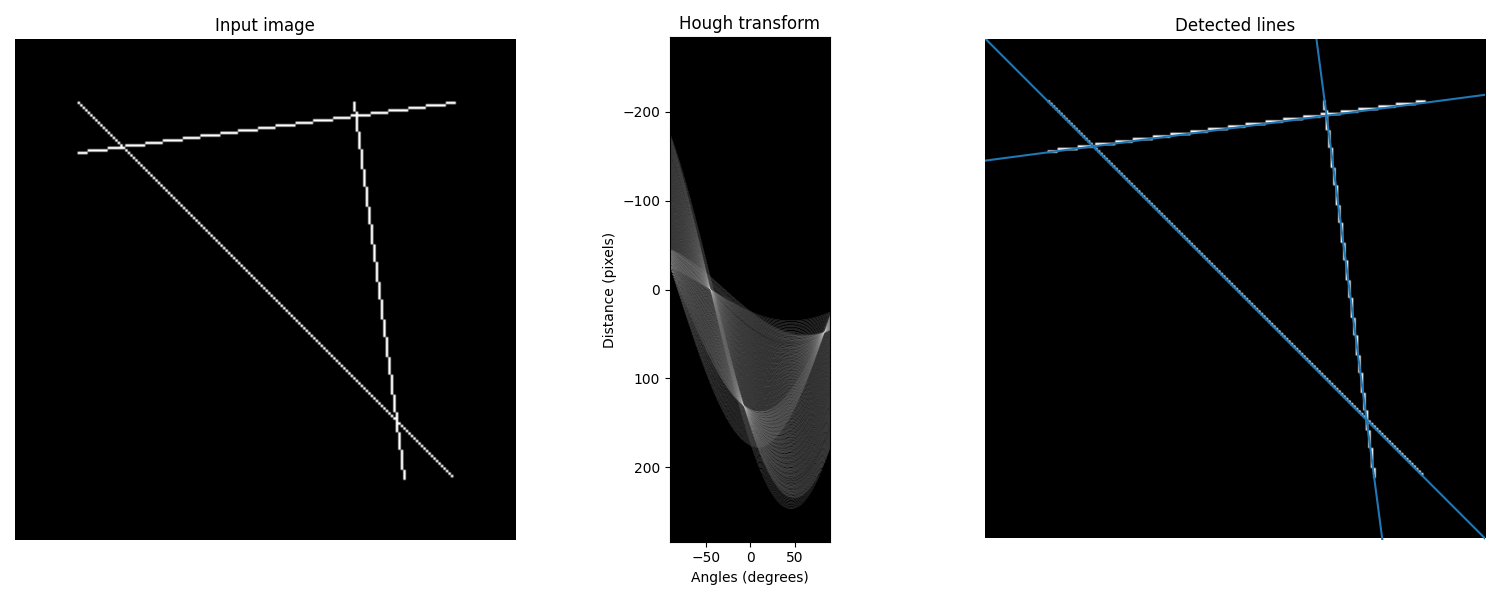
\includegraphics[width=0.5\linewidth]{figures/HoughTransform.png}
    \caption{Hough transform calculation to find the lines of a triangle \cite{hough}}
    \label{fig:houghl}
\end{figure}

\section{Image segmentation algorithms}
\label{sec:ch2sec1}

\subsection{Hough Transform}
\label{subsec:ch2sec1subsec1}

\par This technique was proposed by Paul Hough in 1962, as a method to identify patterns in images. \cite{Duda1972}
\par The Hough Transform is used in computer vision and image processing. The core idea behind it is a voting process made by the curves in the transform space, creating cluster points or local maxima. These points represent the existence of a shape, and since the curves contain the parameters of the shapes, from those parameters the position of the shape in the input image can be detected. 
\par The main strength of this method is that it is capable of identifying shapes even in slightly obscured or noisy data. This made this procedure a massive breakthrough in image processing. Since it's powerful to be able to detect shapes, the method is used in many sectors, from robotic navigation, by identifying edges and lines in the environment, to medical imaging, by detecting circular shapes potentially depicting different biological conditions and many more, where image processing can be utilized.

\subsection{Viola-Jones Face Detection}
\label{subsec:ch2sec1subsec2}
\par Another breakthrough in computer vision was the face detection procedure proposed by Paul Viola and Michael Jones in 2001. \cite{viola2001}
\par The main idea behind their approach lies in the usage of Haar-like feature and Adaptive Boosting.
\par The Haar-like features are simple rectangular regions in the input image data. The main goal of using these patterns is first to cut down on the necessary calculations by working with pixels, and second is to get a better understanding about certain regions in the image. By calculating the differences in the sum of pixel intensities between the regions, a contrast can be learned, an incredibly useful information which allows the detection of basic patterns, like edges, lines and textures.
\par Adaptive boosting is a machine learning algorithm used for boosting weak classifiers into a strong one. The main principle of this method is to iteratively  train weak classifier, each focusing on different features. At each iteration pass, the algorithm selects the best performing classifier and merges it with the final strong one, weight proportionally to its performance. It also weighs incorrectly classified instances more for the next iteration for the purpose of shifting the focus on the most challenging parts.
\par With the help of these two procedures the method of Viola and Jones achieves great accuracy in real-time, more specifically at 15 frames per second on a 700 MHZ Intel Pentium III, using approximately 50 thousand parameters. Since its low hardware requirements, this way of face detection is still used on very weak devices.

\section{Deep learning algorithms}
\label{sec:ch2sec2}
\par With the increase in computational power, image processing algorithms have also evolved in tandem. As seen in the Viola-Jones face detection algorithm, machine learning were already used in the early 2000s, be it at a smaller scale.
\par Since these algorithms now are able to utilize more resources, they can work with way more parameters, going from thousands to millions, allowing them to learn more complex features than before.
\par My choice for the following three deep learning architectures is that, they were significant achievements in the field of computer vision, while also resembling my chosen base model the MobilNet.

\subsection{YOLO}
\label{subsec:ch2sec2subsec1}
\par YOLO (You only live once) is an object detection method, based on a Convolutional Neural Network backbone.
\par The main selling point of this algorithm, is that it achieves real-time performance with a single-pass approach. It divides the image into a grid, each predicting a bounding box, with an associated confidance score and class probability. Utilizing these parameters and various anchor boxes, which are bounding boxes with a predefined shape, size and aspect ratio, the model predicts the final bounding box for the searched cell. \cite{redmon2018yolov3}
\par Since its real-time performance the method has been utilized in many projects, from autonomous driving, to surveillance systems.

\begin{table}[htbp]
\begin{center}
\begin{tabular}
{|p{90pt}|p{90pt}|p{90pt}|p{90pt}|}
\hline
 Type  &  Filters & Size & Output\\
\hline 
\hline Convolutional & $64-1024$ & $3x3/2$ & $128x128-8x8$ \\
\hline Convolutional & $32-512$ & $1x1$ & $ $ \\
\hline Convolutional & $64-1024$ & $3x3$ & $ $ \\
\hline Residual & $ $ & $ $ & $128x128-8x8$ \\
\hline
\end{tabular}
\end{center}
\caption{Building blocks for the YoloV3 CNN backbone, Darknet-53 \cite{redmon2018yolov3}}
\label{YoloTable}
\end{table}

\subsection{RESNET}
\label{subsec:ch2sec2subsec2}
\par ResNet is a convolutional neural network proposed by Kaiming He and co. in 2015, achieving great performances in various computer vision tasks.
\par The main strength of this model is that it addressed the vanishing gradient problem, via the introduction of skip connections. The residual blocks, the main building blocks of this model, contain the shortcut connections, skipping one or more layers. With this, the network is able to learn  residual functions, basically the difference between the desired output and the input data. This feature allows the ResNet architecture to increase the depth of the model, without the gradient vanishing. \cite{he2015deep}

\begin{table}[htbp]
\begin{center}
\begin{tabular}
{|p{120pt}|p{120pt}|}
\hline
Number of layers & Number of parameters\\
\hline 
\hline $20$ & $0.27M$ \\
\hline $32$ & $0.46M$ \\
\hline $44$ & $0.66M$ \\
\hline $56$ & $0.85M$ \\
\hline $110$ & $1.7M$ \\
\hline $1202$ & $19.7M$ \\
\hline
\end{tabular}
\end{center}
\caption{Correlation between the size of the model and the number of parameters used \cite{he2015deep}}
\label{ResNetTable}
\end{table}

\subsection{MOBILENET}
\label{subsec:ch2sec2subsec3}
\par MobileNet is a convolutional neural network designed specifically for mobile and other devices with limited computational power.
\par At its core the architecture is built using depthwise separable convolutions. The standard convolutions is separated into two separated operations. The first one being a depthwise convolution, in which a single convolution filter is applied for each input channel, capturing features separatly. The second is pointwise operations, which applies a 1x1 filter to the outputs of the the previous calculations, combining the results. This allows the model to significantly reduce the number of parameters needed, compared to normal convolution, thus decreasing the computational power needed. \cite{howard2017mobilenets}

\begin{table}[htbp]
\begin{center}
\begin{tabular}
{|p{120pt}|p{120pt}|p{120pt}|}
\hline
Model & ImageNet Accuracy & Parameters\\
\hline 
\hline Conv MobileNet & $71.7\%$ & $29.3M$ \\
\hline MobileNet & $70.6\%$ & $4.2M$ \\
\hline
\end{tabular}
\end{center}
\caption{Difference in parameters between Depthwise separable and full convolutional MobileNet architecture \cite{howard2017mobilenets}}
\label{MobileNetTable}
\end{table}

%Adaugarea și Referirea la o Ecuație \ref{LabelMyEquation}.


 %\begin{equation}
 %    ws_N4 = w_{14}*N1 + W_{24}+N2 + w_{34}*N3
%\label{LabelMyEquation}
% \end{equation}

\chapter{Titlul capitolului}
\label{chap:ch3}

\par Lorem ipsum dolor sit amet, consectetur adipiscing elit, sed do eiusmod tempor incididunt ut labore et dolore magna aliqua. Ut enim ad minim veniam, quis nostrud exercitation ullamco laboris nisi ut aliquip ex ea commodo consequat. Duis aute irure dolor in reprehenderit in voluptate velit esse cillum dolore eu fugiat nulla pariatur. Excepteur sint occaecat cupidatat non proident, sunt in culpa qui officia deserunt mollit anim id est laborum


\section{Sectiune}
\label{sec:ch3sec1}

\par Lorem ipsum dolor sit amet, consectetur adipiscing elit, sed do eiusmod tempor incididunt ut labore et dolore magna aliqua. Ut enim ad minim veniam, quis nostrud exercitation ullamco laboris nisi ut aliquip ex ea commodo consequat. Duis aute irure dolor in reprehenderit in voluptate velit esse cillum dolore eu fugiat nulla pariatur. Excepteur sint occaecat cupidatat non proident, sunt in culpa qui officia deserunt mollit anim id est laborum


\subsection{Subsectiune}
\label{subsec:ch3sec1subsec1}

\par Lorem ipsum dolor sit amet, consectetur adipiscing elit, sed do eiusmod tempor incididunt ut labore et dolore magna aliqua. Ut enim ad minim veniam, quis nostrud exercitation ullamco laboris nisi ut aliquip ex ea commodo consequat. Duis aute irure dolor in reprehenderit in voluptate velit esse cillum dolore eu fugiat nulla pariatur. Excepteur sint occaecat cupidatat non proident, sunt in culpa qui officia deserunt mollit anim id est laborum

\section{Sectiune}
\label{sec:ch3sec2}

\par Lorem ipsum dolor sit amet, consectetur adipiscing elit, sed do eiusmod tempor incididunt ut labore et dolore magna aliqua. Ut enim ad minim veniam, quis nostrud exercitation ullamco laboris nisi ut aliquip ex ea commodo consequat. Duis aute irure dolor in reprehenderit in voluptate velit esse cillum dolore eu fugiat nulla pariatur. Excepteur sint occaecat cupidatat non proident, sunt in culpa qui officia deserunt mollit anim id est laborum


\subsection{Subsectiune}
\label{subsec:ch3sec2subsec1}

\par Lorem ipsum dolor sit amet, consectetur adipiscing elit, sed do eiusmod tempor incididunt ut labore et dolore magna aliqua. Ut enim ad minim veniam, quis nostrud exercitation ullamco laboris nisi ut aliquip ex ea commodo consequat. Duis aute irure dolor in reprehenderit in voluptate velit esse cillum dolore eu fugiat nulla pariatur. Excepteur sint occaecat cupidatat non proident, sunt in culpa qui officia deserunt mollit anim id est laborum


\chapter{Machine learning model specifications}
\label{chap:ch4}

\section{Modified MobileNet}
\label{sec:ch4sec1}

\subsection{Transfer learning specifications}
\label{sec:ch4sec1subsec1}

\subsection{Model output}
\label{sec:ch4sec1subsec2}

\section{Data}
\label{sec:ch4sec2}

\subsection{Data specification}
\label{sec:ch4sec2subsec1}

\subsection{Data preprocessing}
\label{sec:ch4sec2subsec2}
\chapter{Application structure}
\label{chap:ch5}

\section{Graphical User Interface}
\label{sec:ch5sec1}

\section{File Repository}
\label{sec:ch5sec2}

\section{Image processing}
\label{sec:ch5sec3}

\chapter{Performance metrics}
\label{chap:ch6}

\section{Computing machine specifications}
\label{sec:ch6sec1}

\subsection{Training specifications}
\label{sec:ch6sec1subsec1}

\subsection{Running specifications}
\label{sec:ch6sec1subsec2}

\section{Training metrics}
\label{sec:ch6sec2}

\section{Real-time performance}
\label{sec:ch6sec3}

\chapter{Future Work}
\label{chap:ch7}

\section{Machine Learning Model Improvements}
\label{sec:ch7sec1}

\section{GPU Utilization}
\label{sec:ch7sec2}

\chapter{Conclusions}
\label{conclusions}

%\addcontentsline{toc}{chapter}{Concluzii}
%\addcontentsline{toc}{chapter}{Conclusions}

\bibliography{references}

\end{document}
